\chapter{\MakeUppercase{Постановка задачи и план решения}}

\section{Задачи работы}

В рамках работы рассматривается разработка шагающего четырехногого робота, с упором на проблему проектирования конечностей и разработки программного обеспечения для управления движением.

Для выполнения работы требуется:
\begin{itemize}
    \item Разработать общую кинематическую схему робота.
    \item Рассчитать худший (по нагрузке) статический случай для конечностей 4-х ногого робота.
    \item Подобрать электроприводы удовлетворяющие по крутящему моменту.
    \item Подобрать остальные комплектующие (управляющая электроника, детали корпуса, источник питания, проводка), входящие в состав робота и обеспечивающие его автономную работу.
    \item Спроектировать и собрать прототип робота.
    \item Разработать ПО для управления робота.
\end{itemize}

\section{Краткое описание кинематической схемы}

Для поставленных ранее задач можно сформировать последовательность действий для дальнейшей работы. Хотя изначально данных было недостаточно, исходя из опыта были сделаны некоторые предположения по требуемым габаритам конечностей робота и крутящим моментам двигателей, которые в последствии оказались верны.

Далее исходя из дополненных данных о длинах и моментах нужно лишь рассчитать ограничение на массу тела робота, после чего можно продолжать работу. После изучения существующих на рынке роботов, было решено применить в своей конструкции наиболее распрострененное решение. Оптимальной кинематикой можно считать конечность с 3 степенями свободы, как на рисунке \ref{fig:kin_scheme1}.

\begin{figure}[ht]
    \centering
    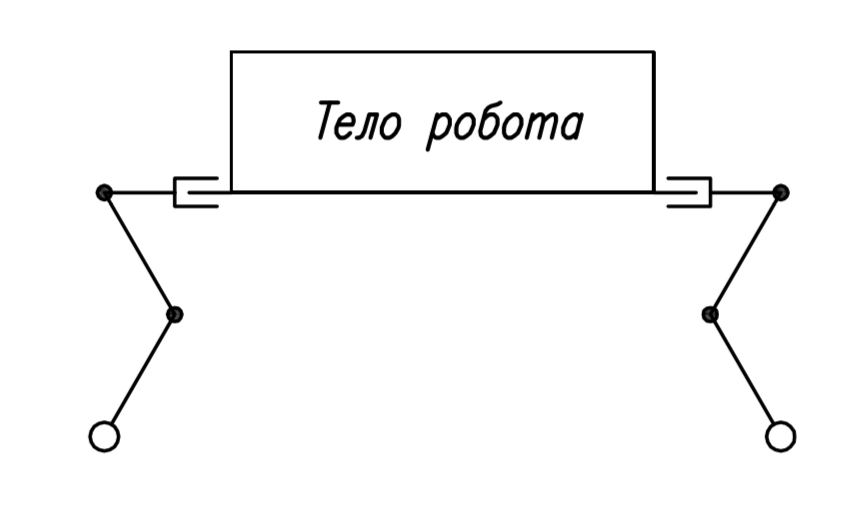
\includegraphics[scale=0.7]{kin1.png}
    \caption{Кинематика 4-х ногого робота, вид сбоку}
    \label{fig:kin_scheme1}
\end{figure}

% \fixme ИЛЛЮСТРАЦИЯ

\subsection{Рассчёт худшего статического случая}

Найдем максимальную статическую нагрузку на приводы конечностей рассмотрев наихудшую статическую конфигурацию робота.

«Худшей» конфигурацией называется такая, при которой одному или нескольким приводам нужно приложить максимальный момент для поворота звена конечности в нужную сторону.

Спроектированные для прототипа конечности имеют длины:
\begin{align*}
    l_1 &\approx = 131\: мм \\
    l_2 &\approx = 134.5\: мм
\end{align*}

Худшим случаем является случай, при котором робот лежит на «животе» с выпрямленными конечностями. Чтобы подогнуть под себя конечность, нужно будет преодолеть момент $M_{худш}$ с учетом массы тела робота $m_T$. При этом максимальный крутящий момент потребуется приводу, находящемуся в первом узле, или можно сказать, управляющему первой степенью свободы.

\begin{figure}[ht]
    \centering
    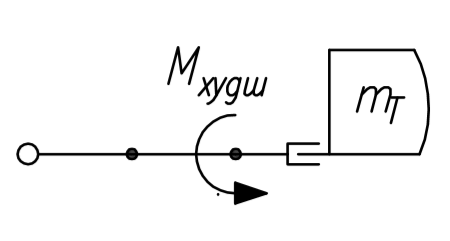
\includegraphics[scale=1]{kin2.png}
    \caption{Кинематика 4-х ногого робота, вид сбоку (худший случай)}
\end{figure}
% на рисунке показать реакцию опоры и mg

При расчёте в первом приближении можно пренебречь трением и весами звеньев. Также можно учесть, что нагрузка, создаваемая массой тела робота будет распределена равномерно по всем 4-м ногам. Это значит что на одну ногу будет приходится лишь $\frac{1}{4}m$ тела робота.

Большая часть веса придется на каркас конструкции, собранный из пластика. Меньшая часть веса придется на аккумулятор. Еще более маленькая часть придется на проводку и крепежи. Самыми легкими составляющими конструкции окажутся электронные компоненты. 
% показать сколько килограмм набирается с комплектующих

При таком расчете можно считать что каждой ноге надо будет «поднять» около 0.25 кг веса. Тогда в худшем случае, приложенный момент вычисляется просто:
$$ M_{худш}= \frac 1 4 (l_{1}+l_{2}) m g, $$
\noindent здесь $l_1$ и $l_2$ - длины звеньев.

Мы можем подобрать длины звеньев таким образом, чтобы они обеспечивали достаточную для задач ходьбы рабочую область и одновременно наименьший требуемый момент.

% перенести ближе к практической конструкторской части
\noindent С использованием приводов с крутящим моментом $ 2.5 \: Н \cdot м $ максимально допустимый вес робота будет примерно равен $ 3.8 \: кг $. Такое требование к весу, с учетом изготовления деталей из аллюминия и пластика, вполне выполнимо.

После получения оценочных данных можно переходить к проектированию основных узлов робота. Результат проектирования показан на рисунке \ref{fig:final_render}.

\begin{figure}[h]
    \centering
    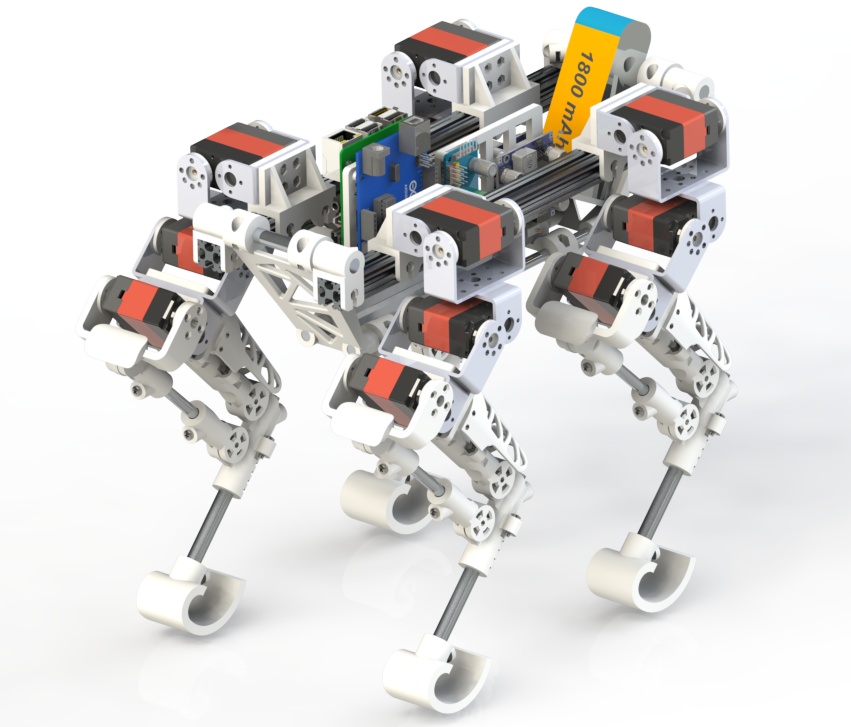
\includegraphics[width=\textwidth]{chapter_mechanics_construction/figure20.png}
    \caption{Сборочный чертеж робота.}
    \label{fig:final_render}
\end{figure}

